% Specify the type of document
\documentclass[12pt]{article}

% Load a number of useful packages
\usepackage{graphicx}
\usepackage{amsmath,amssymb,amsfonts,amsthm}
 \usepackage[margin=1.0in]{geometry}
\usepackage[colorlinks=true]{hyperref}
\usepackage{cite}
\usepackage[caption=false,font=footnotesize]{subfig}
\usepackage{float}

% Two more packages that make it easy to show MATLAB code
\usepackage[T1]{fontenc}
\usepackage[framed,numbered]{matlab-prettifier}
\lstset{
	style = Matlab-editor,
	basicstyle=\mlttfamily\small,
}

% Say where pictures (if any) will be placed
\graphicspath{{./pictures/}}

% Define title, author, and date
\title{AE353: Design Problem 03}
\author{Emilio Gordon}
\date{March, 2017}

% Start of document
\begin{document}

% Put the title, author, and date at top of first page
\maketitle


\section{Goal}
\lstinline!DesignProblem03! simulates an unpowered glider in flight. The glider is designed with an elevator, a control surface which controls an aircraft's pitch during flight. Equipped with an actuator, the elevator's angular rate can be specified. The glider is also equipped with sensors to read both the pitch angle of the craft and the relative angle of the elevator. 
\\ \\
The goal is to make the glider fly the largest range possible if released at a height of approximately two meters with a forward speed of about six meters per second. A requirement for this model is established such that
\begin{itemize}
\item The data of multiple completed simulations will have a mean and median horizontal distance traveled of 20m within a $\pm5\%$ range.
\item The standard deviation for the collected data should be less than 5.
\end{itemize}
With this requirement in mind, a procedure for verification is established. Verification ensures that the system meets the established requirements. Verification will be conducted through several methodologies and are as follows
\begin{itemize}
\item Data will be acquired for up to 1000 flight simulations. This will be done by implementing the script shown in Figure \ref{fig:fgc} on the DesignProblem03 code. 
\item Using Matlab, a histogram can be created in order to visualize the frequency of glider flight distances. 
\item Using Matlab, a minimum, maximum, median, mean and standard deviation can be computed for the acquired data.
\begin{figure}[H]
\begin{quote}
\begin{lstlisting}
% Number of flights
nFlights = 1e3;
% Loop over each flight
for i=1:nFlights
    % Run simulation without graphics and save data
    DesignProblem03('Controller','datafile','data.mat','display',false);
    % Load data
    load('data.mat');
    % Get t and x
    t = processdata.t
    x = processdata.x
    % Do analysis...
    %     (your code here)
end
\end{lstlisting}
\end{quote}
\caption{Flight Generation Code\label{fig:fgc}}
\end{figure}
\end{itemize}
%%%%%%%%%%%%%%%%%%%%%%%%%%%%%%%%%%%%%%%%%%%%%%%%%%%%%%%%
%                                                                                 Model                                                                                  %
%%%%%%%%%%%%%%%%%%%%%%%%%%%%%%%%%%%%%%%%%%%%%%%%%%%%%%%%
\section{Model}
The motion of the glider is governed by ordinary differential equations with the form
\begin{equation}
\label{eqEOM}
\begin{bmatrix} \ddot{x} \\ \ddot{z} \\ \ddot{\theta} \end{bmatrix} = f(\theta,\phi,\dot{x},\dot{z},\dot{\theta},\dot{\phi})
\end{equation}
where $\theta$ is the pitch angle, $\phi$ is the elevator angle, $\dot{x}$ is the forward speed, $\dot{z}$ is the vertical speed, $\dot{\theta}$ is the pitch angular rate, and $\dot{\phi}$ is the elevator angular rate.  $\dot{\phi}$ is the only parameter which can be defined by the user. 
\\ \\
The equations of motion were derived by applying the a flat-plate model of lift $c_{L}$ and drag $c_{D}$ as a function of angle of attack $\alpha$, for both the wing and elevator:
\begin{equation*}
c_{L} = 2\sin\alpha \cos\alpha
\qquad\qquad
c_{D} = 2\sin^{2}\alpha
\end{equation*}
Experimental results show that this flat-plate model is a good approximation for the glider and that it remains accurate at high angles of attack and even post-stall \cite{Moore2014}. 
\\ \\
The function $f$ in Equation \eqref{eqEOM} depends on a number of parameters (e.g., mass, moment of inertia, surface area of the wing) which can be represented symbolically within the controller code (\lstinline|Controller.m|). The equations of motion are first loaded into the controller using the following code which was provided in \lstinline!DesignProblem03! documentation.
\begin{figure}[H]
\begin{quote}
\begin{lstlisting}
% Load the equations of motion.
load('DesignProblem03_EOMs.mat');
% Parse the equations of motion.
f = symEOM.f;
% Define symbolic variables that appear in the equations of motion.
syms theta phi xdot zdot thetadot phidot
\end{lstlisting}
\end{quote}
\end{figure}
The first step to a standard approach of control design is linearizing the nonlinear equations of motion about an equilibrium point. In order to accomplish this, an equilibrium point must first be found by setting the equations of motion to 0. In other words, a solution to
\begin{equation*}
0 = f(\theta,\phi,\dot{x},\dot{z},0,0).
\end{equation*}
must be found. However due to the complexity with the derived equations of motion, this equation was solved for numerically in MATLAB using the function \lstinline|fsolve|.The following code presented in Figure \ref{fig:equill} was graciously provided by Dr. T. Bretl of the University of Illinois via Piazza post @216.
\begin{figure}[H]
\begin{quote}
\begin{lstlisting}
% INPUTS:
% f is a symbolic description of the nonlinear EOMs
%   (theta, phi, xdot, zdot) is a guess at the equilibrium point
% OUTPUTS:
%   (theta, phi, xdot, zdot) is an equilibrium point near the guess
function [theta,phi,xdot,zdot] = GetEquilibriumPoint(f,theta,phi,xdot,zdot)
% Initial guess
x0 = [theta;phi;xdot;zdot];
% Symbolic states
syms theta phi xdot zdot thetadot real
% Symbolic inputs
syms phidot real
% Symbolic EOMs with thetadot=0 and phidot=0
g = subs(f,[thetadot,phidot],[0,0]);
% Numeric EOMs
vars = [theta;phi;xdot;zdot];
g = matlabFunction(g,'Vars',{vars});
% Find solution
xe = fsolve(g,x0)
% Parse solution
theta = xe(1)
phi = xe(2)
xdot = xe(3)
zdot = xe(4)
end
\end{lstlisting}
\end{quote}
\caption{Equilibrium Calculation Script\label{fig:equill}}
\end{figure}
The script in Figure \ref{fig:equill} produces equilibrium values for $\theta$, $\phi$, $\dot{x}$ and $\dot{z}$ when $\theta$, $\phi$, $\dot{x}$, $\dot{z}$ were defined to be 0,0,6,0 respectively. Additional equilibrium values are manually defined. Those are the equilibrium values for $\dot{\theta}$ and $\dot{\phi}$, both of which are zero. Overall, the equilibrium state and equilibrium input for the system are defined in Equation \eqref{equil}.
\begin{equation}
\label{equil}
eq_{\textrm{state}} = 
\begin{bmatrix}
\dot{x_{e}} \\ \dot{z_{e}} \\ \dot{\theta_{e}} \\  \theta_{e} \\ \phi_{e}
\end{bmatrix}
=
\begin{bmatrix}
6.0973 \\ -0.5488 \\ 0 \\ 0.0046 \\ -0.0660
\end{bmatrix}
\quad
eq_{\textrm{input}} = 
\begin{bmatrix}
\dot{\phi_{e}}
\end{bmatrix}
=
\begin{bmatrix}
0
\end{bmatrix}
\end{equation}
It should be mentioned that through the process of finding an equilibrium point, a state, input and output were defined. Shown in Equation \eqref{sys}, the system has five states, one input and two outputs. For the case of state, $x$ and $z$ are not included since they do not appear on the right hand side of the equation of motion in Equation \eqref{eqEOM}.
\begin{equation}
\label{sys}
\textrm{state} = 
\begin{bmatrix}
\dot{x} \\ \dot{z} \\ \dot{\theta} \\  \theta \\ \phi
\end{bmatrix}
\quad
\textrm{input} = 
\begin{bmatrix}
\dot{\phi}
\end{bmatrix}
\quad
\textrm{output} = 
\begin{bmatrix}
\theta \\ \phi
\end{bmatrix}
\end{equation}
Having acquired the equilibrium points and defined a state, input and output for the system, a linear model can now be produced.  These calculations were conducted utilizing Matlab's symbolic toolbox. 
\\
\begin{figure}[!h]
\begin{quote}
\begin{lstlisting}
%Define State and Input
state = [xdot; zdot; thetadot; theta; phi];
input = [phidot];
%Linearization
A = double([vpa(subs(jacobian(fsym,state),[state; input],[eqstate; eqinput]))]);
B = double(vpa(subs(jacobian(fsym,input),[state; input],[eqstate; eqinput])));
C = [0 0 0 1 0;0 0 0 0 1];
\end{lstlisting}
\end{quote}
\caption{Symbolic Linearization Script\label{fig:linear}}
\end{figure} 
\\
The results to the section of code in Figure \ref{fig:linear} are shown in Equation Set \eqref{eqnJacob} which contain the matrices A, B and C for the state-space model. The D matrix is simply 0 since the output does not rely on the input of the system.
\\
\begin{equation}
\begin{aligned}
\label{eqnJacob} 
%{\left(\begin{bmatrix} {qdd}_{e} \end{bmatrix}, x_{eqil}\right)}
A =& \begin{bmatrix} 
-0.0035  & -0.1037  &  0.0606 &  -8.7700   &  0.8012 \\ 0.8741 & -32.4187 & 1.8124 & 324.6115 & 64.9536 \\ 0.5048 &  15.1038  & -8.8301 & -151.5407 & -216.5083 \\0     &    0   & 1.0000    &     0     &    0 \\0    &     0    &     0    &     0    &     0

\end{bmatrix}
\\ \\
 %{\left(\begin{bmatrix} {qdd}_{e} \end{bmatrix}, x_{eqil}\right)} 
B =& 
\begin{bmatrix} 
  0.0074 \\
    0.3238 \\
   -1.0795 \\
         0 \\
    1.0000
\end{bmatrix} 
\qquad \qquad \qquad \qquad \qquad \; \;
%{\left(\begin{bmatrix} {qdd}_{e}\end{bmatrix}, x_{eqil}\right)}
C =
\begin{bmatrix} 1 & 0 & 0 & 0 & 0\\ 0 & 1 & 0 & 0 & 0 \\ 0 & 0 & 1 & 0 & 0 \\ 0 & 0 & 0 & 1 & 0 \\ 0 & 0 & 0 & 0 & 1\end{bmatrix}
\end{aligned}
\end{equation}
\\ \\
The resulting state-space model is
\begin{align*}
\dot{x} &= Ax+Bu \\
y &= Cx
\end{align*}
such that the behavior of this linear system and of the original, nonlinear system will be approximately the same so long as the system is close to equilibrium.
%%%%%%%%%%%%%%%%%%%%%%%%%%%%%%%%%%%%%%%%%%%%%%%%%%%%%%%%
%                                                                              Cont.+Obs.                                                                             %
%%%%%%%%%%%%%%%%%%%%%%%%%%%%%%%%%%%%%%%%%%%%%%%%%%%%%%%%
\section{Controller and Observer}
The system is a simple aircraft model that can be described as a single rigid body subject to gravitation and aerodynamic forces. In the previous section, a space-state model was derived by computing linear model around a set of equilibrium points for the equations of motion described in equation \eqref{eqEOM}. To obtain the desired performance, it is required to test for controllability and observability.  This is critical for the analysis of a system before deciding the best control strategy to be applied, or whether it is even possible to control or stabilize the system. 
%%%%%%%%%%%%%%%%%%%%%%%%%%%%%%%%%%%%%%%%%%%%%%%%%%%%%%%%
%                                                                               Controller                                                                              %
%%%%%%%%%%%%%%%%%%%%%%%%%%%%%%%%%%%%%%%%%%%%%%%%%%%%%%%%
\subsection{Controller}
Controllability refers to a systems ability to reach a particular state through an appropriate control input. In designing a controller, the system must be verified for controllability and stability. If a state is controllable, then the system can be told to reach a certain state and is considered stable. However, if the system is not controllable, no input will be able to control the state. Even if the state is not controllable, the dynamics may still be stable, resulting in a stable state. The MATLAB code in Figure \ref{fig:cont} completes these objectives.
\begin{figure}[!h]
\begin{quote}
\begin{lstlisting}
%Verfies System is Controllable
abs(rank(ctrb(A,B))-length(A))

%Define Gains Controller
Qc = [10000 0 0 0 0;0 1000 0 0 0;0 0 1000 0 0;0 0 0 1 0;0 0 0 0 1];
Rc = 1;
K = lqr(A,B,Qc,Rc);

%Verifies if Controller is Asymptoticly Stable
eig(A-B*K)
\end{lstlisting}
\end{quote}
\caption{Controller\label{fig:cont}}
\end{figure}
\\
The code insures the system is controllable by validating controllability and stability. Controllability is verified in the second line of code in Figure \ref{fig:cont}. The output of this line results can be either
\begin{itemize}
\item 0: The rank is equivalent to the size of the A matrix and results in 0, confirming controllability.
\item 1: The rank is not equivalent to the size of the A matrix and results in 1, disproving controllability. 
\end{itemize}
After proving controllability, a linear feedback control design based on Quadratic Regulators (LQR) is implemented. Implementing LQR introduces a Q and R matrix. The Q matrix represents the cost on the state while the R matrix is the cost on the action. The selected Q and R matrices are represented in Equation \eqref{qnr}. Through LQR, a K matrix can be found as shown in line seven of Figure \ref{fig:cont}.
\\ \\
\begin{equation}
\begin{aligned}
\label{qnr}
 %{\left(\begin{bmatrix} {qdd}_{e} \end{bmatrix}, x_{eqil}\right)} 
Q =& 
\begin{bmatrix} 1 & 0 & 0 & 0 & 0\\ 0 & 1 & 0 & 0 & 0 \\ 0 & 0 & 1 & 0 & 0 \\ 0 & 0 & 0 & 1 & 0 \\ 0 & 0 & 0 & 0 & 1\end{bmatrix}
\qquad \qquad
%{\left(\begin{bmatrix} {qdd}_{e}\end{bmatrix}, x_{eqil}\right)}
R =&
\begin{bmatrix} 1\end{bmatrix}
\end{aligned}
\end{equation}
\\ \\
Finally, with the controllability verified and gain defined, controller stability must now be computed. Stability is verified in line 10 of code in Figure \ref{fig:cont}. The eigenvectors of the matrix computation,  $A-BK$, must have negative real parts.
\\ \\
\begin{equation} \label{eqiCont} \begin{aligned}
\textrm{eig(A-BK)} = \begin{bmatrix}-62.44 +57.06i\\ -62.44 -57.06i\\ -3.317\\ -8.969\\ -27.82\\
\end{bmatrix} \end{aligned} \end{equation}
\\ \\
Since Equation \eqref{eqiCont} has negative real parts, stability is confirmed and the controlled is complete.
%%%%%%%%%%%%%%%%%%%%%%%%%%%%%%%%%%%%%%%%%%%%%%%%%%%%%%%%
%                                                                               Observer                                                                               %
%%%%%%%%%%%%%%%%%%%%%%%%%%%%%%%%%%%%%%%%%%%%%%%%%%%%%%%%
\subsection{Observer}
Observability relates to the possibility of observing the state of a system, via output sensor measurements. In designing an observer, the system must be verified for observability and stability, similar to designing a controller. If a state is not observable, the controller will never be able to predict the behavior of an unobservable state and therefore, is unable to be stabilized. However, a system that is not observable may still be stable.
\begin{figure}[!h]
\begin{quote}
\begin{lstlisting}
%Verifies System is Observable
rank(obsv(A,C))-length(A)

%Define Gains Observer
Qo = [1 0; 0 1];
Ro = [1 0 0 0 0;0 1 0 0 0;0 0 1 0 0;0 0 0 1 0;0 0 0 0 1];
L = lqr(A',C',inv(Ro),inv(Qo))';

%Verifies if Observer is Asymptoticly Stable
eig(A-L*C)
\end{lstlisting}
\end{quote}
\caption{Observer\label{fig:obsv}}
\end{figure}
The code insures the possibility of an observer by validating observability and stability. Observability is verified in the second line of code in Figure \ref{fig:obsv}. The output of this line results can be either
\begin{itemize}
\item 0: The rank is equivalent to the size of the A matrix and results in 0, confirming observability.
\item 1: The rank is not equivalent to the size of the A matrix and results in 1, disproving observability. 
\end{itemize}
After proving observability, a linear feedback control design based on Quadratic Regulators (LQR) is implemented much like what was done for the controller. Implementing LQR introduces a Q and R matrix where the Q matrix represents the cost on the state and the R matrix represents the cost on the action. The selected Q and R matrices are represented in Equation \eqref{qnro}. Through LQR, an L matrix can be found as shown in line seven of Figure \ref{fig:obsv}.
\\ \\
\begin{equation}
\begin{aligned}
\label{qnro}
 %{\left(\begin{bmatrix} {qdd}_{e} \end{bmatrix}, x_{eqil}\right)} 
Q =& 
\begin{bmatrix} 1 & 0 \\ 0 & 1\end{bmatrix}
\qquad \qquad
%{\left(\begin{bmatrix} {qdd}_{e}\end{bmatrix}, x_{eqil}\right)}
R =&
\begin{bmatrix} 1 & 0 & 0 & 0 & 0\\ 0 & 1 & 0 & 0 & 0 \\ 0 & 0 & 1 & 0 & 0 \\ 0 & 0 & 0 & 1 & 0 \\ 0 & 0 & 0 & 0 & 1\end{bmatrix}
\end{aligned}
\end{equation}
\\ \\
Finally, with the observability verified and a gain defined, controller stability must now be computed. Stability is verified in line 10 of code in Figure \ref{fig:obsv}. The eigenvectors of the matrix computation,  $A-LC$, must have negative real parts.
\\ \\
\begin{equation} \label{eqObsv} \begin{aligned}
\textrm{eig(A-LC)} = \begin{bmatrix}
-24.46\\ -16.89\\ -2.663 + 2.740i\\ -2.663 - 2.740i\\ -0.048
\end{bmatrix} \end{aligned} \end{equation}
\\ \\
Since Equation \eqref{eqObsv} has negative real parts, stability is confirmed and the observer is complete.
\section{Implementation}
With controllability and observability successfully verified, a controller can be implemented into the system. This section will go into detail the setup of the controller. First, a Zero-Input controller will be demonstrated to serve as control data set, a comparison for future test. Second, the controller will be demonstrated and explained. Finally, a comparison between the two will be made.
%%%%%%%%%%%%%%%%%%%%%%%%%%%%%%%%%%%%%%%%%%%%%%%%%%%%%%%%
%                                                                              Zero-Input                                                                              %
%%%%%%%%%%%%%%%%%%%%%%%%%%%%%%%%%%%%%%%%%%%%%%%%%%%%%%%%
\subsection{Zero-Input System}
A zero-input system has no inputs. This means the value being put into the actuators is simply zero. No force or actuation is occurring so the system will behave in its most natural sense. This is an important observation to keep in mind, especially after the controller is applied. It is expected that the controller will operate more efficiently than the zero-input system and therefore, makes a good basis for how well the controller behaves. 
\\
\begin{lstlisting}[frame=single]
actuators.phidot = 0;
\end{lstlisting}
\\ \\ 
\begin{figure}[H]
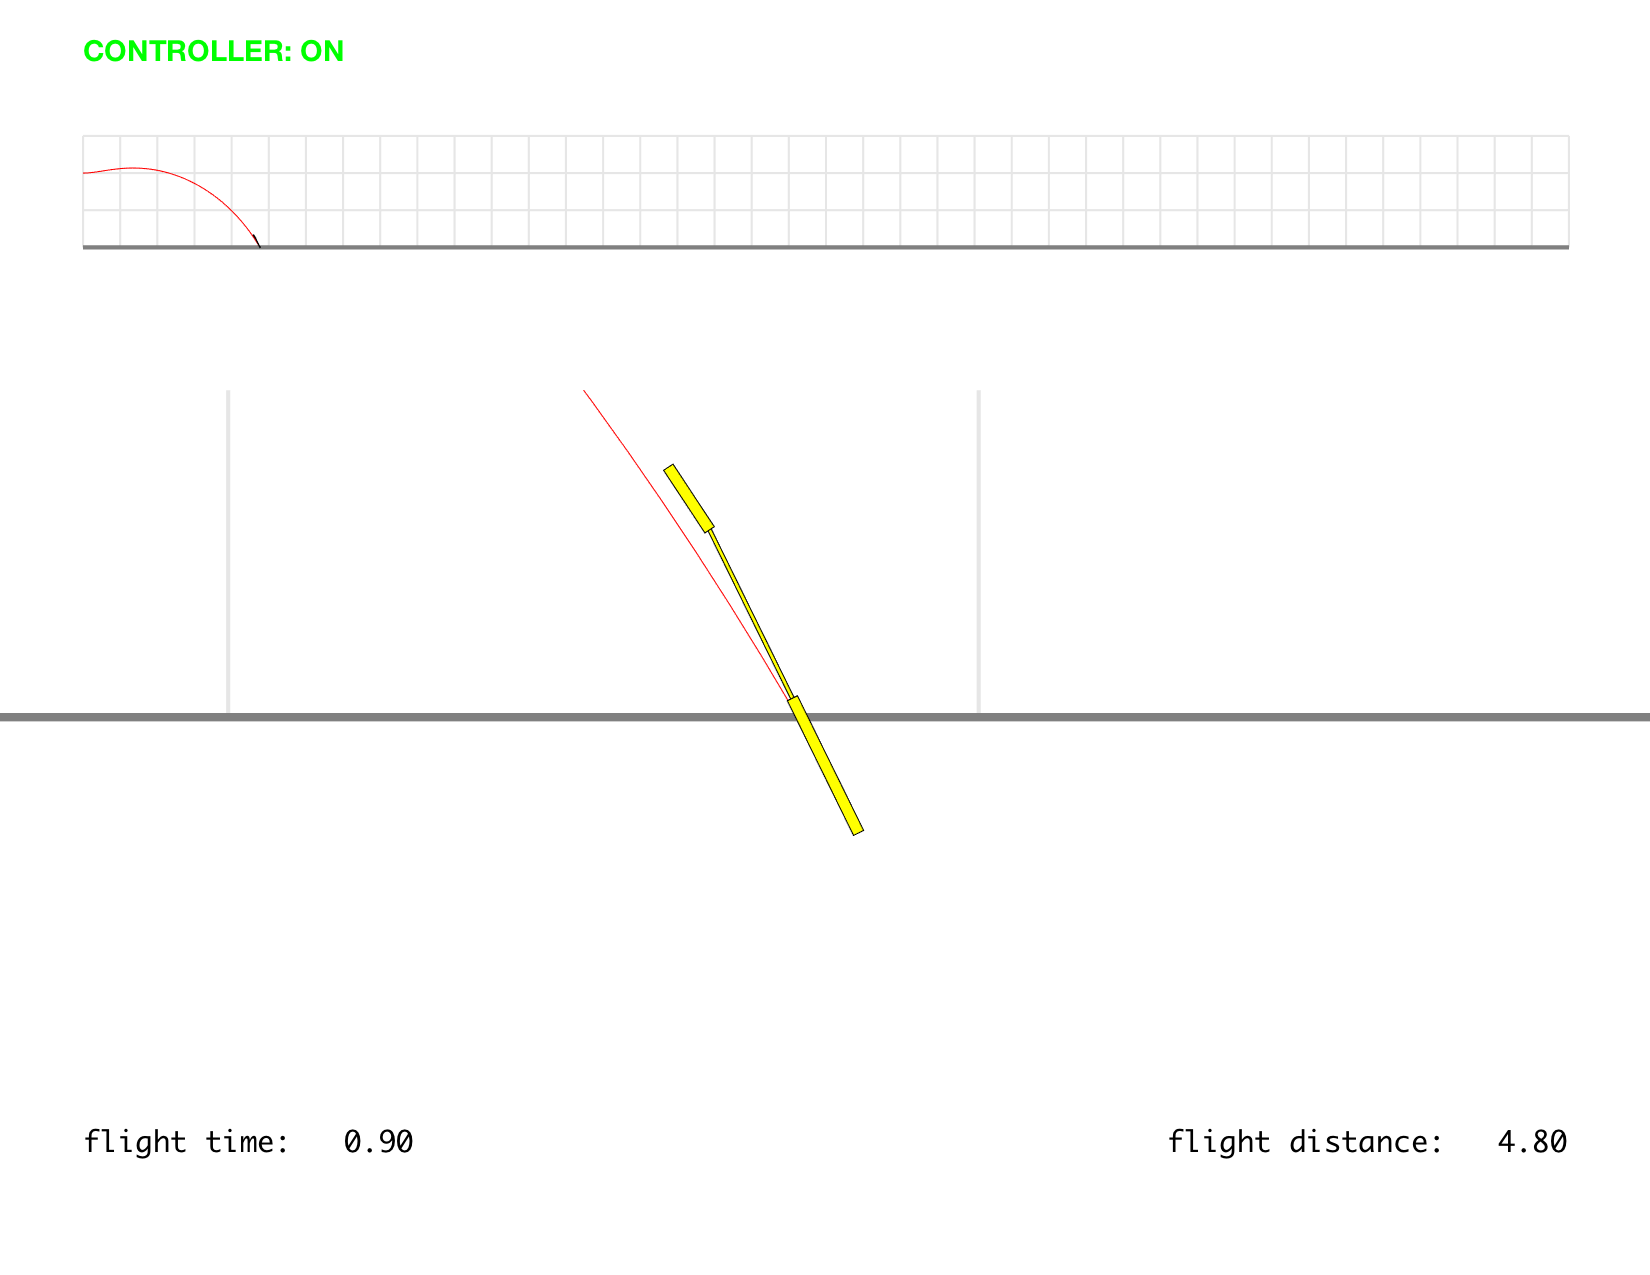
\includegraphics[width=1\textwidth]{zeroinput.pdf}
\centering
\caption{Flight Path and Simulated Model with Zero Input}
\label{zi}
\end{figure} 
\\ \\
As can be seen with Figure \ref{zi}, the glider carried out with the initial random velocity it was assigned and proceeded to plummet to a vertical height of zero.
\\ \\
\begin{table}[H]
\centering
\begin{tabular}{|p{4cm}|p{4cm}|p{4cm}|}
\hline
Property & Matlab Code & Output \\
\hline \hline
Minimum  & $\lstinline|min|$ & 0.4241\\
Maximum &   $\lstinline|max|$ & 25.6775\\
Median & $\lstinline|std|$ & 5.4965\\ 
Mean    & $\lstinline|mean|$ & 7.0362\\ 
Standard Deviation &   $\lstinline|std|$  & 4.4895\\
\hline
\end{tabular}
\caption{Matlab Data Summary for Zero Input\label{zeroTable}}
\end{table}
\\ \\
For the purposes of having comparable data, the procedure defined in the verifications section is conducted. The results of which are the histogram in Figure \ref{zeroHist} and the data summary in Table \ref{zeroTable}.
\\ \\
\begin{figure}[H]
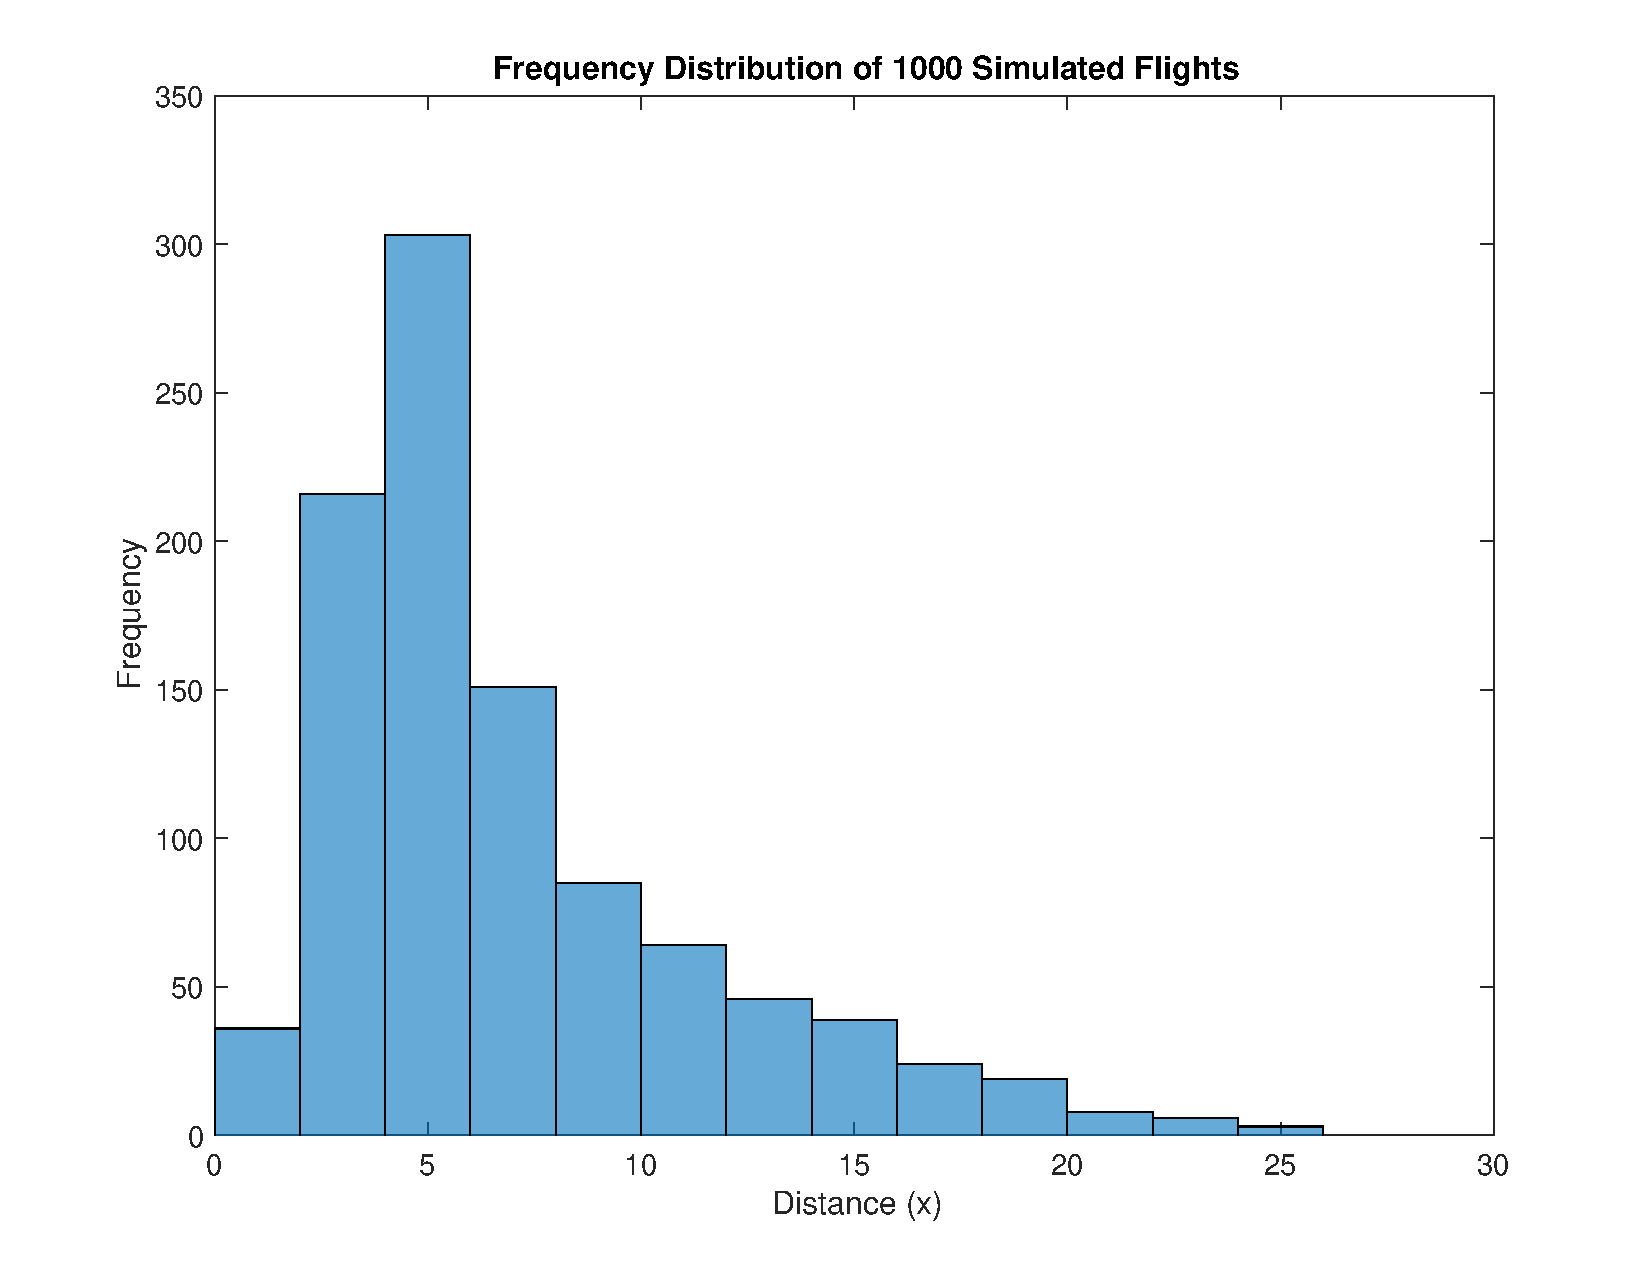
\includegraphics[width=1\textwidth]{zeroHist.pdf}
\caption{Frequency distribution of flight distance for 1000 simulated flights with zero-input}
\label{zeroHist}
\end{figure}
%%%%%%%%%%%%%%%%%%%%%%%%%%%%%%%%%%%%%%%%%%%%%%%%%%%%%%%%
%                                                                               Controller                                                                              %
%%%%%%%%%%%%%%%%%%%%%%%%%%%%%%%%%%%%%%%%%%%%%%%%%%%%%%%%
\subsection{Closed Loop System}
It was seen that through a zero-input system, the model will behave under no forces or dynamic changes. In the following section, a controller using state-feedback and state-estimation is implemented. The sensors that are accessible are $\phi$, the elevator pitch, and $\theta$, the glider pitch. Note that the defined state in Equation \eqref{sys} has a total of five states however, only two states can be collected from the gliders sensors. To resolve this, an observer is created in order to generate a state estimate that would closely represent the missing data. 
\\ \\
Since C was defined as a $2x5$ matrix, it is important to define the output as the two states the system can contribute.
\begin{lstlisting}[frame=single]
%Define Sensor Values
theta = sensors.theta;
phi = sensors.phi;
%Establish Output
output = [theta; phi];
\end{lstlisting}
Using the sensor values, the output of the system must be corrected in terms of the equilibrium values.
\begin{lstlisting}[frame=single]
%WHAT?
y = output - C*[eqstate];
\end{lstlisting}
Now that the output of the system has been defined, focus is placed on the input. The input, as for any closed-loop system is simply 
\begin{lstlisting}[frame=single]
%Input using estimated state
u =-K*xhat;
\end{lstlisting}
$\hat{x}$ which represents the state estimation, was previously defined as $[0; 0; 0; 0; 0]$ but is subject to change after the first iteration. To accomplish this the change in state estimation, $\dot{\hat{x}}$ is computed.
\begin{lstlisting}[frame=single]
%Next step for dxhat
dxhat = A*xhat+B*u-L*(C*xhat-y);
\end{lstlisting}
With $\dot{\hat{x}}$ now known, Euler's method can be used to find $\hat{x}$, the estimate for the state. This is later applied in the next iteration affecting the input.
\begin{lstlisting}[frame=single]
%Euler's Method for finding xhat
data.xhat = xhat + h*dxhat;
\end{lstlisting}
With all these calculation made, an input can confidently be implemented into the actuator. The actuators must be corrected by adding the equilibrium input. For the case of this system, the correction factor is simply zero. 
\begin{lstlisting}[frame=single]
%Applying controller to the input
actuators.phidot = u+eqinput;
\end{lstlisting}

%%%%%%%%%%%%%%%%%%%%%%%%%%%%%%%%%%%%%%%%%%%%%%%%%%%%%%%%
%                                                                                Analysis                                                                                %
%%%%%%%%%%%%%%%%%%%%%%%%%%%%%%%%%%%%%%%%%%%%%%%%%%%%%%%%
\section{Analysis}
\label{secAnalysis}
Since the initial conditions for the glider are random every iteration, one test will not suffice in accomplishing the goal. For a given control design, the flight distance will vary across a wider ranger. Therefore, data from at least 1000 flights must be conducted. Using the code in Figure \ref{fig:fgc}, the data for 1000 flights was carried out. 
\begin{figure}[H]
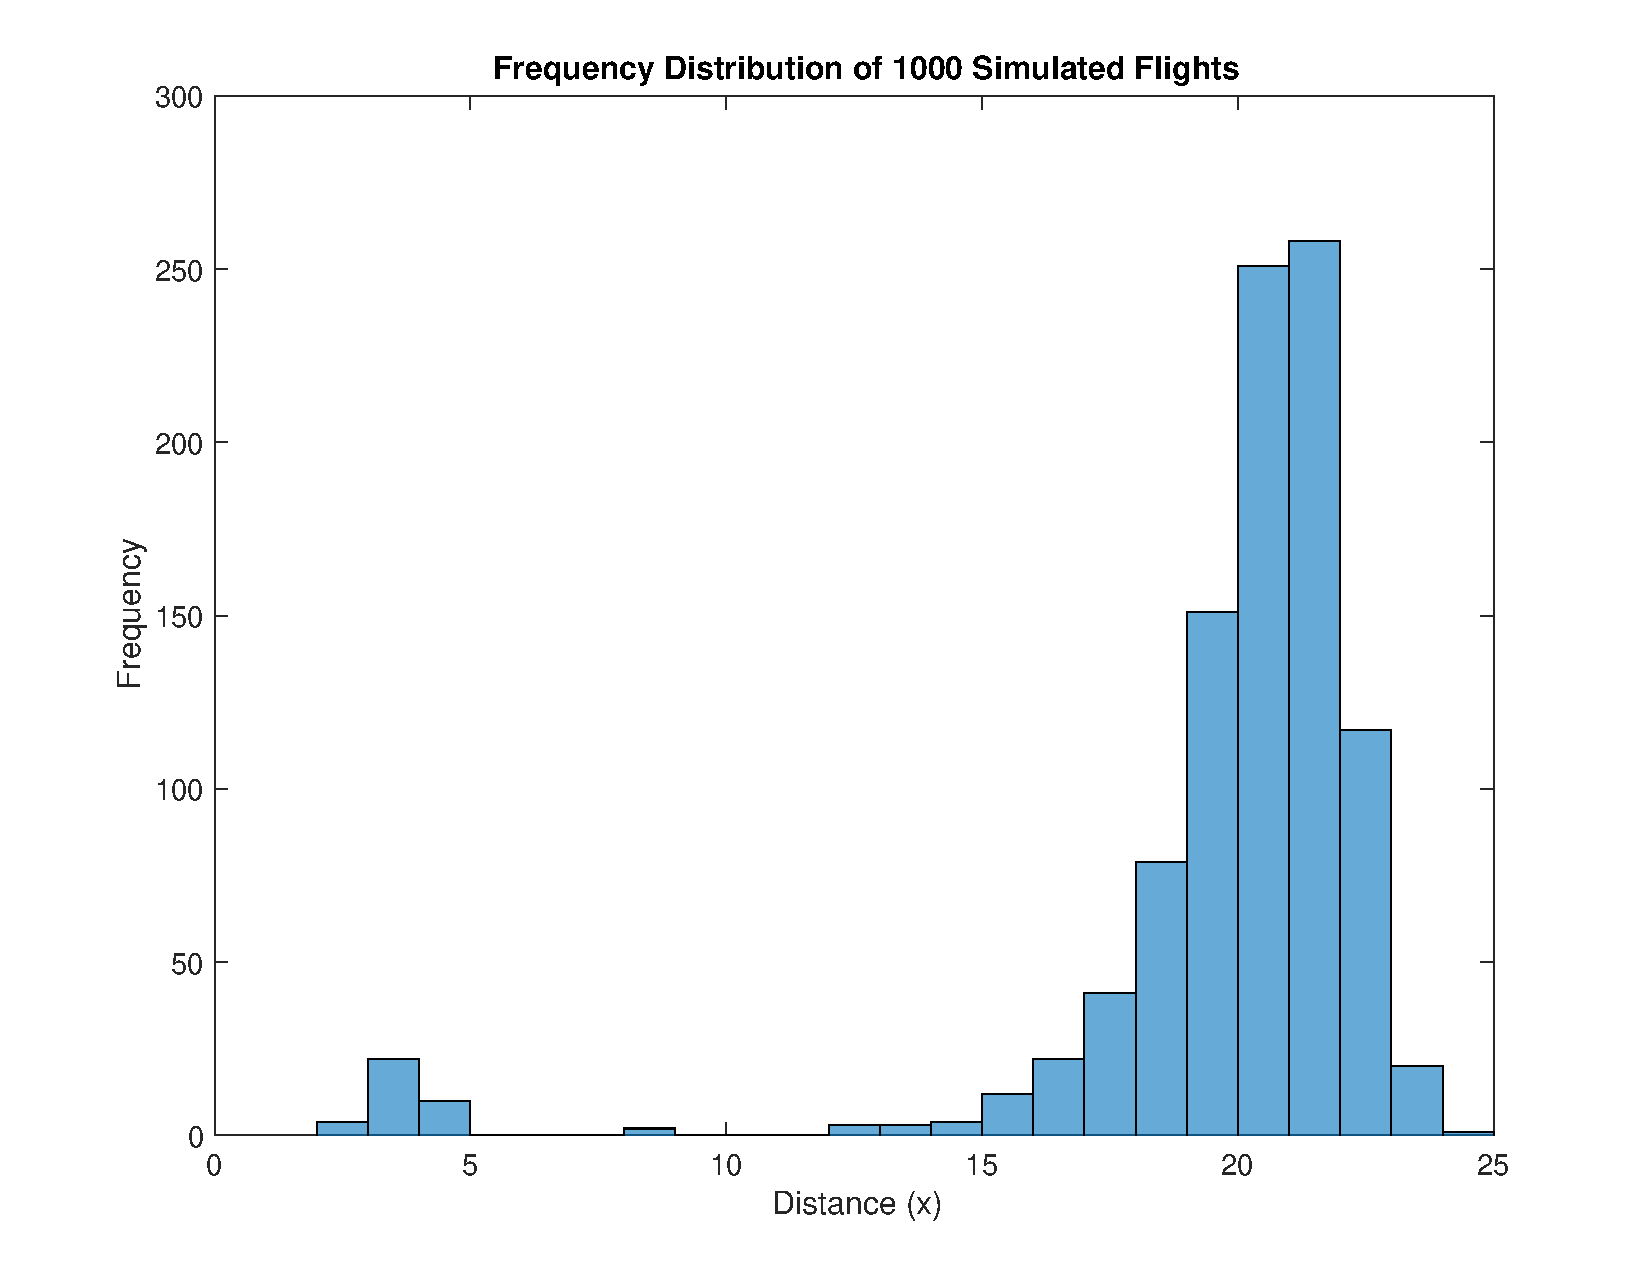
\includegraphics[width=1\textwidth]{flights1.pdf}
\caption{Frequency distribution of the total flight distance for 1000 simulated flights}
\label{hist}
\end{figure}
Following the procedure set by the verifications, the minimum, maximum, median, mean, and standard deviation of the flight distance. The table \ref{table:1} provides the results of the data collected from the script and its associated matlab function.
 
\begin{table}[H]
\centering
\caption{Matlab Data Summary\label{table:1}} \\ 
\begin{tabular}{|p{4cm}|p{4cm}|p{4cm}|}
\hline
Property & Matlab Code & Output \\
\hline \hline
Minimum  & $\lstinline|min|$ & 2.034712540102511\\
Maximum &   $\lstinline|max|$ & 24.511317632554807\\
Median & $\lstinline|std|$ & 20.628279007621781\\ 
Mean    & $\lstinline|mean|$ & 19.770135217421497\\ 
Standard Deviation &   $\lstinline|std|$  & 3.572052578055217\\
\hline
\end{tabular}
\end{table}
This can be compared to the zero-input model. It is clear that the controller had significant improvements to the gliders ability to reach a farther distance. In fact, the glider implementing the controller has an average distance approximately four times more effective than the glider with zero-input. This is expected of course but serves as a good indication to the success of the controller.

% Display list of references in IEEE Transactions format.
\bibliographystyle{IEEEtran}
\bibliography{IEEEabrv,references}

% End of document (everything after this is ignored)
\end{document}